% Options for packages loaded elsewhere
\PassOptionsToPackage{unicode}{hyperref}
\PassOptionsToPackage{hyphens}{url}
%
\documentclass[
  english,
  man,floatsintext]{apa6}
\usepackage{lmodern}
\usepackage{amsmath}
\usepackage{ifxetex,ifluatex}
\ifnum 0\ifxetex 1\fi\ifluatex 1\fi=0 % if pdftex
  \usepackage[T1]{fontenc}
  \usepackage[utf8]{inputenc}
  \usepackage{textcomp} % provide euro and other symbols
  \usepackage{amssymb}
\else % if luatex or xetex
  \usepackage{unicode-math}
  \defaultfontfeatures{Scale=MatchLowercase}
  \defaultfontfeatures[\rmfamily]{Ligatures=TeX,Scale=1}
\fi
% Use upquote if available, for straight quotes in verbatim environments
\IfFileExists{upquote.sty}{\usepackage{upquote}}{}
\IfFileExists{microtype.sty}{% use microtype if available
  \usepackage[]{microtype}
  \UseMicrotypeSet[protrusion]{basicmath} % disable protrusion for tt fonts
}{}
\makeatletter
\@ifundefined{KOMAClassName}{% if non-KOMA class
  \IfFileExists{parskip.sty}{%
    \usepackage{parskip}
  }{% else
    \setlength{\parindent}{0pt}
    \setlength{\parskip}{6pt plus 2pt minus 1pt}}
}{% if KOMA class
  \KOMAoptions{parskip=half}}
\makeatother
\usepackage{xcolor}
\IfFileExists{xurl.sty}{\usepackage{xurl}}{} % add URL line breaks if available
\IfFileExists{bookmark.sty}{\usepackage{bookmark}}{\usepackage{hyperref}}
\hypersetup{
  pdftitle={Comparing probabilistic accounts of probability judgments},
  pdfauthor={Derek Powell1},
  pdflang={en-EN},
  pdfkeywords={keywords},
  hidelinks,
  pdfcreator={LaTeX via pandoc}}
\urlstyle{same} % disable monospaced font for URLs
\usepackage{graphicx}
\makeatletter
\def\maxwidth{\ifdim\Gin@nat@width>\linewidth\linewidth\else\Gin@nat@width\fi}
\def\maxheight{\ifdim\Gin@nat@height>\textheight\textheight\else\Gin@nat@height\fi}
\makeatother
% Scale images if necessary, so that they will not overflow the page
% margins by default, and it is still possible to overwrite the defaults
% using explicit options in \includegraphics[width, height, ...]{}
\setkeys{Gin}{width=\maxwidth,height=\maxheight,keepaspectratio}
% Set default figure placement to htbp
\makeatletter
\def\fps@figure{htbp}
\makeatother
\setlength{\emergencystretch}{3em} % prevent overfull lines
\providecommand{\tightlist}{%
  \setlength{\itemsep}{0pt}\setlength{\parskip}{0pt}}
\setcounter{secnumdepth}{-\maxdimen} % remove section numbering
% Make \paragraph and \subparagraph free-standing
\ifx\paragraph\undefined\else
  \let\oldparagraph\paragraph
  \renewcommand{\paragraph}[1]{\oldparagraph{#1}\mbox{}}
\fi
\ifx\subparagraph\undefined\else
  \let\oldsubparagraph\subparagraph
  \renewcommand{\subparagraph}[1]{\oldsubparagraph{#1}\mbox{}}
\fi
% Manuscript styling
\usepackage{upgreek}
\captionsetup{font=singlespacing,justification=justified}

% Table formatting
\usepackage{longtable}
\usepackage{lscape}
% \usepackage[counterclockwise]{rotating}   % Landscape page setup for large tables
\usepackage{multirow}		% Table styling
\usepackage{tabularx}		% Control Column width
\usepackage[flushleft]{threeparttable}	% Allows for three part tables with a specified notes section
\usepackage{threeparttablex}            % Lets threeparttable work with longtable

% Create new environments so endfloat can handle them
% \newenvironment{ltable}
%   {\begin{landscape}\centering\begin{threeparttable}}
%   {\end{threeparttable}\end{landscape}}
\newenvironment{lltable}{\begin{landscape}\centering\begin{ThreePartTable}}{\end{ThreePartTable}\end{landscape}}

% Enables adjusting longtable caption width to table width
% Solution found at http://golatex.de/longtable-mit-caption-so-breit-wie-die-tabelle-t15767.html
\makeatletter
\newcommand\LastLTentrywidth{1em}
\newlength\longtablewidth
\setlength{\longtablewidth}{1in}
\newcommand{\getlongtablewidth}{\begingroup \ifcsname LT@\roman{LT@tables}\endcsname \global\longtablewidth=0pt \renewcommand{\LT@entry}[2]{\global\advance\longtablewidth by ##2\relax\gdef\LastLTentrywidth{##2}}\@nameuse{LT@\roman{LT@tables}} \fi \endgroup}

% \setlength{\parindent}{0.5in}
% \setlength{\parskip}{0pt plus 0pt minus 0pt}

% \usepackage{etoolbox}
\makeatletter
\patchcmd{\HyOrg@maketitle}
  {\section{\normalfont\normalsize\abstractname}}
  {\section*{\normalfont\normalsize\abstractname}}
  {}{\typeout{Failed to patch abstract.}}
\patchcmd{\HyOrg@maketitle}
  {\section{\protect\normalfont{\@title}}}
  {\section*{\protect\normalfont{\@title}}}
  {}{\typeout{Failed to patch title.}}
\makeatother
\shorttitle{Comparing probability judgment accounts}
\keywords{keywords\newline\indent Word count: X}
\usepackage{csquotes}
\usepackage{tikz}
\usetikzlibrary{bayesnet}
\ifxetex
  % Load polyglossia as late as possible: uses bidi with RTL langages (e.g. Hebrew, Arabic)
  \usepackage{polyglossia}
  \setmainlanguage[]{english}
\else
  \usepackage[shorthands=off,main=english]{babel}
\fi
\ifluatex
  \usepackage{selnolig}  % disable illegal ligatures
\fi
\newlength{\cslhangindent}
\setlength{\cslhangindent}{1.5em}
\newlength{\csllabelwidth}
\setlength{\csllabelwidth}{3em}
\newenvironment{CSLReferences}[2] % #1 hanging-ident, #2 entry spacing
 {% don't indent paragraphs
  \setlength{\parindent}{0pt}
  % turn on hanging indent if param 1 is 1
  \ifodd #1 \everypar{\setlength{\hangindent}{\cslhangindent}}\ignorespaces\fi
  % set entry spacing
  \ifnum #2 > 0
  \setlength{\parskip}{#2\baselineskip}
  \fi
 }%
 {}
\usepackage{calc}
\newcommand{\CSLBlock}[1]{#1\hfill\break}
\newcommand{\CSLLeftMargin}[1]{\parbox[t]{\csllabelwidth}{#1}}
\newcommand{\CSLRightInline}[1]{\parbox[t]{\linewidth - \csllabelwidth}{#1}\break}
\newcommand{\CSLIndent}[1]{\hspace{\cslhangindent}#1}

\title{Comparing probabilistic accounts of probability judgments}
\author{Derek Powell\textsuperscript{1}}
\date{}


\authornote{

Arizona State University, School of Social and Behavioral Sciences

The authors made the following contributions. Derek Powell: Conceptualization, Writing - Original Draft Preparation, Writing - Review \& Editing.

}

\affiliation{\vspace{0.5cm}\textsuperscript{1} Arizona State University, School of Social and Behavioral Sciences}

\abstract{
Bayesian theories of cognitive science hold that cognition is fundamentally probabilistic. However, one mark sometimes held against these theories is that people's explicit probability judgments often violate the laws of probability. Two recent proposals, the ``Probability Theory plus Noise'' (Costello \& Watts, 2014) and ``Bayesian Sampler'' (Zhu, Sanborn, \& Chater, 2020) theories of probability judgments, both seek to account for these biases while maintaining that mental credences are fundamentally probabilistic. These theories fit quite differently into the larger project of Bayesian cognitive science, but their many similarities complicate comparisons of their predictive accuracy. In particular, comparing the models demands a careful accounting of model complexity. Here, I cast these theories into a Bayesian data analysis framework that supports principled model comparison using information criteria. Compared the fits of both models on data collected by Zhu and colleagues (2020) I find the data are best explained by a modified version of the Bayesian Sampler model that allows for informative priors.
}



\begin{document}
\maketitle

Bayesian theories and approaches offer a unified formal framework for cognitive science (Tenenbaum, Kemp, Griffiths, \& Goodman, 2011) that has had remarkable successes across domains, including in perception (e.g. Kersten, Mamassian, \& Yuille, 2004), memory (Anderson, 1991), language (Xu \& Tenenbaum, 2007), and reasoning (Lu, Chen, \& Holyoak, 2012). At the heart of the Bayesian project is the idea that cognition is fundamentally probabilistic: that people reason according to subjective degrees of belief which follow the laws of probability and, in particular, that they are revised in light of evidence according to Bayes' Rule. It is somewhat embarrassing then, that that these theories have often been accused of failing to describe human ``beliefs'' of the simple and everyday sort, such as beliefs like ``it will rain tomorrow,'' ``vaccines are safe,'' or ``this politician is trustworthy.''

Trouble starts as soon as we seek to measure beliefs. According to Bayesian theories of cognition and epistemology (Jaynes, 2003), the degree to which people believe in various propositions, or their credences, should reflect subjective mental probabilities. So asking people to express beliefs in terms of probability seems only natural.

Unfortunately, people's explicit probability judgments routinely violate the axioms of probability theory. For example, human probability judgments often exhibit the ``conjunction fallacy'': people will often judge the conjunction of two events (e.g.~``Tom Brady likes football and miniature horses'') as being more probable than one of the events in isolation (e.g.~``Tom Brady likes miniature horses''), a plain and flagrant violation of probability theory (Tversky \& Kahneman, 1983). Other demonstrations of the incoherence of probability judgments include disjunction fallacies, subadditivity or ``unpacking'' effects (Tversky \& Koehler, 1994), and a variety of other effects illustrating the incoherence of human probability judgments (for an accessible review, see Kahneman, 2013). Altogether these findings have led many researchers to abandon the notion that degrees of belief are represented as probabilities.

Recently however, two groups of researchers have proposed theories of human probability judgments that account for biases and apparent incoherence in these judgments while maintaining that mental credences are fundamentally probabilistic (Costello \& Watts, 2014; Zhu, Sanborn, \& Chater, 2020). Both of these theories build on the increasingly popular notion that a variety of human reasoning tasks are accomplished by a limited process of mental ``sampling'' from a probabilistic mental model (see also Chater et al., 2020; Dasgupta, Schulz, \& Gershman, 2017).

\hypertarget{two-probabilistic-theories-of-probability-judgment}{%
\subsection{Two probabilistic theories of probability judgment}\label{two-probabilistic-theories-of-probability-judgment}}

Costello \& Watts (2014, 2016, 2018) have proposed a theory of probability judgment they call the ``Probability Theory plus Noise'' theory (PT+N). In the PT+N model, mental ``samples'' are drawn from a probabilistic mental model of events and are then ``read'' with noise, so that some positive examples will be read as negative and some negative examples read as positive. The results are probability judgments reflecting probabilistic credences perturbed by noise. In their model, the probability a mental sample for an event \(A\) is read as A is the probability that the sample truly is A, p(A), and that it is correctly read (1-d), plus the probability that the sample is not A, 1-P(A) and that it is incorrectly read (d), or:

\begin{align*}
  P(\text{read as A}) &= (1-d)P(A) + d(1-P(A)) \\
  &= (1-2d)P(A) + d
\end{align*}

Thus under the simplest form of the PT+N model, the expected value of probability judgments is:

\[E[\hat{P}_{PT+N}(A)] = (1-2d)P(A) + d \]

where \emph{d} represents the probability with which samples will be misread, or the amount of noise in the judgment process. By assumption, a maximum of 50\% of samples can be misread, so that d is a number in the range {[}0, .50{]}. The PT+N theory provides a unified accounts for a wide variety of biases in probability judgment that were previously attributed to different types of heuristics (Costello \& Watts, 2014, 2016, 2017, 2018).

Meanwhile, Zhu, Sanborn, \& Chater (2020) have proposed a Bayesian model of probability judgment they call the ``Bayesian Sampler.'' Under this model, probability judgment is itself seen as a process of Bayesian inference. To judge the probability of an event, a limited number of samples are again drawn from a mental model of the event. Then, those ``observed'' samples are integrated with a prior over probabilities to produce a probability judgment. The \(N\) mentally-observed samples are integrated with a Bayesian prior over probabilities, represented with a symmetric Beta distribution parameterized by \(\beta\). After observing \(S(A)\) successes and \(N - S(A)\) failures, this posterior is distributed \(Beta(\beta + S(A), \beta + N - S(A))\). Zhu and colleagues (2020) assume that people report the mean of their posterior probability estimates. Since for any Beta distribution \(x \sim Beta(a,b)\), \(E[x] = \frac{a}{a+b}\), the probability estimate is thus a linear function of S, N, and \(\beta\).

\[\hat{P}_{BS}(A) = \frac{S(A)}{N+2\beta} + \frac{\beta}{N+2\beta}\]

The expected value of the estimate can then be written in terms of the expected number of successes, or \(P(A) \cdot N\). Under the simplest version of the Bayesian Sampler model, this gives the following formula:

\[E[\hat{P}_{BS}(A)] = \frac{N}{N+2\beta}P(A) + \frac{\beta}{N+2\beta}\]

Like the PT+N model, the Bayesian Sampler model accounts for a wide array of biases in probability judgments, including the novel biases identified by Costello and Watts (Costello \& Watts, 2014, 2016). In fact, important equivalencies can be drawn between the two models. Zhu and colleagues (2020) show that the \(N\) and \(\beta\) parameters of their model can be related to the \(d\) parameter of the PT+N model via the following bridging formula:

\[d = \frac{\beta}{N+2\beta}\]

Thus, the effect of a Bayesian prior is nearly identical to the effect of noise in the PT+N model. But, rather than merely perturbing people's probability judgments, this prior can be seen as regularizing these judgments away from extreme values. Zhu and colleagues (2020) argue that such regularization can be adaptive in cases where only a small number of mental samples can be drawn. For instance, consider someone estimating the probability that they can swim across a lake, outrun an animal, or win a hand of poker: if a mental simulation of these events produces two samples indicating success, a person incorporating no other information might conclude these are all certain victories and thereby be too willing to assume risk. A regularizing prior pushes these estimates away from extremes, thereby promoting better decision-making when mental samples are sparse. However, this hedging comes at the cost of systematic incoherence and biases.

\hypertarget{two-accounts-of-conditional-probability-judgments}{%
\subsubsection{Two accounts of conditional probability judgments}\label{two-accounts-of-conditional-probability-judgments}}

By explaining the incoherence of human probability judgments using coherent mental probabilities, both models have the potential to rescue the larger project of Bayesian cognitive science as applied to everyday beliefs (Chater et al., 2020). And the bridging condition identified by Zhu and colleagues (Zhu, Sanborn, \& Chater, 2020) demonstrates that the theories make identical predictions in many cases. However, the two models diverge substantially in their treatment of conditional probability judgments. Bayesian cognitive theories are fundamentally theories of inductive reasoning: Bayes' rule describes how existing beliefs should be updated conditional on the observation of different kinds of evidence. So, how they treat the conditioning of beliefs is at the heart of these theories.

According to the Bayesian sampler model, conditioning is something that happens in the mental model of the events, not as part of the process of rendering probability judgments. By not assigning any special status to conditional probability judgments, the Bayesian Sampler theory fits neatly into the larger Bayesian project of cognitive science: probability judgments are simply another judgment process applied to the outputs of other (ideally Bayesian) mental models (Chater et al., 2020).

In contrast, the PT+N model presents a constructive account of conditional probability judgments that is fundamentally non-Bayesian (Costello \& Watts, 2016). According to the PT+N model, conditional probabilities P(A\textbar B) are estimated by a two-stage sampling procedure: first both events A and B are sampled with noise, and then a second noisy process computes the ratio of the events read as A and B over events read as B. The PT+N model predicts conditional probability estimates using the following equation:

\[P_e(A|B) = \frac{(1-2d)^2P(A \land B) + d(1-2d)\big(P(A)+P(B)\big)+d^2}{(1-2d)P(B)+d}\]

The PT+N's account of conditional probability judgment is distinctly non-Bayesian, thereby separating it from the Bayesian Sampler theory quite fundamentally. In addition, drawing conditioning out of the mental models of events and into the conditional probability judgment process makes it unclear how the PT+N theory would interface with other probabilistic models of cognitive processes that invoke Bayes' rule.

\hypertarget{comparing-the-models}{%
\subsection{Comparing the models}\label{comparing-the-models}}

Zhu, Sanborn, and Chater (2020) compared their Bayesian Sampler model against Costello \& Watts' (2014; 2016; 2017; 2018) PT+N model as explanations for human probability judgments in two experiments. Unfortunately, their results were somewhat equivocal. They fit both ``simple'' and ``complex'' versions of each model and computed a Bayesian Information Criteria score (BIC) for all models. The complex versions of these models introduce additional parameters d' and N' that allow for different patterns of judgments for conjunctive and disjunctive judgments as compared with simple probability judgments. These additional parameters are crucial to both models' explanations of conjunction fallacies---key findings in the probability judgment literature (Costello \& Watts, 2017; Zhu, Sanborn, \& Chater, 2020). Table 1 below presents the total BIC scores computed for each model as originally fit, using the authors' original code and saved model outputs (Zhu, Sanborn, \& Chater, 2020, Supplementary materials).

\begin{table}

\caption{\label{tab:table1}Original model fitting results}
\centering
\begin{tabular}[t]{lrr}
\toprule
Model & Exp. 1 & Exp. 2\\
\midrule
\textbf{Bayesian Sampler simple} & \textbf{956.9} & \textbf{-5371.9}\\
Bayesian Sampler complex & 1174.4 & -5099.3\\
PT+N simple & 1257.5 & -4901.1\\
PT+N complex & 1039.7 & -5159.6\\
Bayesian Sampler avg. & 1065.6 & -5235.6\\
\addlinespace
PT+N avg. & 1148.6 & -5030.4\\
\bottomrule
\end{tabular}
\end{table}

In both experiments, the simple version of the Bayesian Sampler scores best, but the complex version of the PT+N model comes in second (lower BIC scores are better). It is not obvious what conclusions should be drawn from these results. Of course, the simple Bayesian Sampler model appears to win by the numbers. But conjunction fallacies are an extremely robust empirical finding (Mellers, Hertwig, \& Kahneman, 2001; Sides, Osherson, Bonini, \& Viale, 2002) and are clearly present in the data collected by Zhu and colleagues (2020). So we might justifiably rule out the simple variants of the models on the grounds that they will fail to capture important qualitative features of the data, which would instead favor the PT+N theory. For their part, Zhu and colleagues (2020) elect to split the baby by averaging the simple and complex model scores together. This approach somewhat favors the Bayesian Sampler theory overall, though they are cautious about drawing any strong conclusions in favor of their theory.

\hypertarget{accounting-for-model-complexity}{%
\subsubsection{Accounting for Model Complexity}\label{accounting-for-model-complexity}}

When comparing and selecting models based on their predictive accuracy, it is necessary to correct for the potential for these models to ``overfit'' the data. Typically this correction comes in the form of a ``complexity penalty,'' penalizing models in proportion to their flexibility for accommodating different patterns of data (Gelman, Hwang, \& Vehtari, 2014). Zhu and colleagues (2020) warn that BIC, which penalizes models based only on the number of parameters in the model, cannot fully account for the differences in the models' complexity.

There are at least three challenges to accounting for model complexity in the comparison of the PT+N and Bayesian Sampler models. First, the models differ not only in the number of parameters but in the domain of those parameters. Zhu and colleagues (2020) assume that the Bayesian Sampler model's prior distribution should reflect ignorance or a lack of information. A uniform prior, Beta(1, 1) is the most obvious choice in this case, but theoretical arguments can also be made for Beta(0.5, 0.5) (Jeffrey's prior), Beta(0,0) (Haldene's prior), or perhaps other symmetric beta distributions Beta(\(\beta\),\(\beta\)) with \(beta \leq 1\) (Jaynes, 2003). Thus, they restrict the range of the \(\beta\) parameter in their Bayesian Sampler model to fall within the interval {[}0,1{]}. Via the bridging conditions, they show that this restricts the ``noise level'' for the Bayesian Sampler, represented in implied d under the PT+N model, to {[}0, \(1/3\){]}. The Bayesian Sampler's implied \(d\) approaches the upper limit of \(1/3\) as \(N\) approaches \(\infty\) and \(\beta\) equals 1, whereas the PT+N model permits noise values between {[}0, 0.50{]}.

Second, it is not immediately clear how the models' structural differences impact their flexibility. To be sure, Zhu and colleagues' (2020) bridging condition makes it clear that the PT+N model is more flexible when it comes to predicting unconditional probabilities. But, what impact does the PT+N model's treatment of conditional probabilities have on model complexity? Is this component of the model a sort of Ptolemaic epicycle, adding complexity to the model that should be penalized? Or, does it constitute a commitment to novel predictions that thereby constrain its flexibility? Determining model complexity a priori is not always straightforward when the models being compared differ structurally.

Finally, one potential explanation for the relative weakness of the complex model versions is Zhu and colleagues' (2020) use of ``unpooled'' models, where parameters are estimated independently for each individual participant. Adding a parameter for each participant may effectively over-penalize the complex variants relative to the simple variants, especially if there is actually limited heterogeneity across participants. In contrast, a comparison of fully pooled variants of the simple and complex models (where a single population parameter is used for all participants) would require adding only one extra parameter to the penalty term. Partial pooling is a solution that balances between these extreme approaches, allowing for an accounting of heterogeneity without over-penalizing in cases where heterogeneity is low.

\hypertarget{the-present-work}{%
\subsubsection{The present work}\label{the-present-work}}

Here, I cast both the Bayesian Sampler and PT+N models into a Bayesian data analysis framework that may permit a more decisive comparison. First, Bayesian data analysis allows issues of model complexity to be addressed through comparisons of model fit based on information criteria, such as \(WAIC\) and \(LOO_{ic}\). Both of these indices approximate leave-one-out cross validation, thereby offering a measure of the ability of a model to capture new unseen data. Importantly, these indices also allow for complexity penalties that directly capture differences in the flexibility of the models, rather than being estimated based solely on the number of distinct parameters (Gelman, Hwang, \& Vehtari, 2014; Vehtari, Gelman, \& Gabry, 2017). In addition, the Bayesian framework also supports straightforward implementation of hierarchical versions of these models with partial pooling. This allows for information about model parameters to be shared across participants, resulting in a potential reduction in model complexity and a more realistic test of the models.

\hypertarget{methods}{%
\section{Methods}\label{methods}}

\hypertarget{data-selection}{%
\subsection{Data selection}\label{data-selection}}

Zhu, Sanborn, \& Chater (2020) conducted two experiments to compare the PT+N and Bayesian sampler theories. These experiments asked participants to judge the probability of different events in various combinations. Following prior work by Costello and Watts (e.g. 2016, 2018), both experiments focused on the everyday events of different kinds of weather.

Experiment 1 asked about the events {[}icy, frosty{]} and {[}normal, typical{]} (e.g.~``what is the probability that the weather in London is normal and not typical?''). The authors' goal was to ask about highly correlated events, but the events used are perhaps nearly perfectly correlated. Because the terms used to describe these events are nearly synonymous, there is a concern about the interpretation of the statements evaluated in this experiment. This is especially clear, as the authors note, for disjunctive trials such as ``normal or typical,'' where ``or typical'' might not be read as a disjunction but rather an elaborative clause. In light of these concerns, I excluded the disjunctive trials from Experiment 1 from my analyses.

Experiment 2 focused on more moderately correlated events, {[}cold, rainy{]} and {[}windy, cloudy{]}, that do not admit these misinterpretations. In addition, a third experimental condition asking about {[}warm, snowy{]} was also included in the experiment, but was dropped from the analyses reported in the paper. Exploring the raw responses from this condition reveals a substantial fraction of ``zero'' and ``one'' responses for certain trials. This may reflect a different response process than was intended. For instance, some participants may have engaged in deductive reasoning to judge that it is not possible for the weather to at once be warm and snowy, and therefore responded with zero---failing to properly consider that it is possible (at least logically) for it to be warm and snowy at different times within the same day. Given these potentially aberrant responses, I followed Zhu and colleagues (2020) in ignoring data from this condition.

\hypertarget{modeling}{%
\subsection{Modeling}\label{modeling}}

I implement both the Bayesian Sampler and PT+N models as Bayesian models in the probabilistic programming language Numpyro. All code and results are available as supplemental materials (\url{https://github.com/derekpowell/bayesian-sampler}).

\hypertarget{bayesian-implementations-of-the-models}{%
\subsubsection{Bayesian implementations of the models}\label{bayesian-implementations-of-the-models}}

The PT+N model defines probability judgments as:

\begin{align*}
  P_{e}(A) &= (1-2d)P(A) + d \\
  P_e(A\land B) &= (1-d^\prime)P(A \land B)+d^\prime \\
  P_e(A\lor B) &= (1-d^\prime)P(A \lor B)+d^\prime \\
  P_e(A|B) &= \frac{(1-2d)^2P(A \land B) + d(1-2d)\big(P(A)+P(B)\big)+d^2}{(1-2d)P(B)+d}
\end{align*}

In contrast, the Bayesian Sampler model defines probability judgments as:

\begin{align*}
  P_{e}(A) &= \frac{N}{N + 2 \beta}P(A) + \frac{\beta}{N+2 \beta} \\
  P_{e}(A \land B) &= \frac{N’}{N’ + 2 \beta}P(A \land B) + \frac{\beta}{N’+2 \beta} \\
  P_{e}(A \lor B) &= \frac{N’}{N’ + 2 \beta}P(A \lor B) + \frac{\beta}{N’+2 \beta} 
\end{align*}

Fixing d and d' or N and N' equal yields the ``simple'' variant of each of the models, which treat conjunctive and disjunctive probability judgments identically to simple probability judgments.

Notice that for each model the probability judgments depend on underlying subjective probabilities, derived from a mental sampling process. These subjective probabilities are unobserved, and must be estimated as a latent variable. Here, they are represented with a four-dimensional dirichlet distribution for each subject, representing the probability of the elementary events (\(A \land B\), \(\neg A \land B\), \(A \land \neg B\), \(\neg A \land \neg B\)).

Zhu, Sanborn \& Chater (2020) implement completely unpooled models with separate d, d', N, N', and \(\beta\) parameters for each participant. Figure 1 displays the translation of the PT+N model into the Bayesian framework, along with a plate diagram representing the dependencies among parameters.

\begin{figure}
  \begin{minipage}{.5\textwidth}
    \flushright
    \begin{figure}
  \begin{minipage}{.5\textwidth}
    \flushright
    \begin{tikzpicture}

     % Define nodes
     \node[obs]                               (y) {$y_{ijk}$};
     \node[det, above=of y] (mu) {$\mu_{ijk}$};
     \node[det, above=of mu, xshift=-1.2cm]  (d) {$d_j$};
     \node[det, above=of mu, xshift=1.2cm]  (d_prime) {$d_j'$};
     \node[latent, above=of d]  (delta) {$\delta_j$};
     \node[latent, above=of d_prime]  (delta_delta) {$\Delta\delta_j$};
     \node[latent, right=2cm of y]  (kappa) {$\kappa$};
     \node[latent, left=1cm of mu]            (p) {$\vec{p_{jk}}$};

     % Connect the nodes
     \edge {mu, kappa} {y} ; %
     \edge {d, d_prime} {mu}
     \edge {delta} {d, d_prime}
     \edge {delta_delta} {d_prime}
     \edge {p} {mu}

     % Plates
     {
       \tikzset{plate caption/.append style={below=15pt of #1.south east}};
       \tikzstyle{plateIJK} = [align=center];
       \plate[inner sep=0.25cm, xshift=-.0625cm] {plateIJK} {(mu)(y)} {$i$} ;
    }
     {
       \tikzset{plate caption/.append style={above right=0pt of #1.north east}};
       \plate[inner sep=0.25cm, xshift=-.12cm, yshift=-.12cm] {plateJ} {(mu)(y)(p)(d)(d_prime)(delta)(delta_delta)} {$j$} ;
     }
     {
       \tikzset{plate caption/.append style={above right=0pt and 0pt of #1.north west}};
       \plate[inner sep=0.25cm] {plateIJ} {(p)(mu)(y)} {$k$};
     }

   %   \plate {} {(mu)(y)(p)(mup.north west)(mup.south west)} {$M$} ;

\end{tikzpicture}
  \end{minipage}%
  \begin{minipage}{.5\textwidth}
    \flushleft
    \small
    \begin{align*}
      y_{ijk} &\sim Beta\big(\mu_{ijk} \kappa, (1-\mu_{ijk}) \kappa \big) \\
      \mu_{ijk} &= f_{PT+N}(\overrightarrow{p_{jk}}, d_j, d_j)  \\
      d_j &= \frac{1}{2} \ \text{logistic}(\delta_j) \\
      d_j’ &= \frac{1}{2} \ \text{logistic}\big(\delta_j + \exp(\Delta\delta_j)\big) \\
      \overrightarrow{p_{jk}} &\sim Dirichlet(\overrightarrow{1}) \\
      \delta_j &\sim Normal(0,1) \\
      \Delta\delta_j &\sim Normal(0,1) \\
      \kappa &\sim \mathit{Half \hyph Cauchy}(20)
    \end{align*}
  \end{minipage}
  \caption{Complex unpooled PT+N model diagram and formula specifications. Circular nodes are parameters, shaded nodes are observations, and squared nodes are deterministic functions of parameters. Plates signify values defined for $i$ trials, $j$ participants, and $k$ conditions.}
\end{figure}



  \end{minipage}%
  \begin{minipage}{.5\textwidth}
    \flushleft
    \small
    \begin{align}
      y_{ijk} &\sim beta\big(\mu_{ijk} \kappa, (1-\mu_{ijk}) \kappa \big) \\
      \mu_{ijk} &= f_{PT+N}(\overrightarrow{p_{jk}}, d_j, d_j)  \\
      d_j &= \frac{expit(\delta_j)}{2} \\
      d_j’ &= \frac{expit\big(\delta_j + \exp(\Delta\delta_j)\big)}{2} \\
      \overrightarrow{p_{jk}} &\sim Dirichlet(\overrightarrow{1}) \\
      \delta_j &\sim Normal(0,1) \\
      \Delta\delta_j &\sim Normal(0,1) \\
      \kappa &\sim HalfCauchy(20)
    \end{align}
  \end{minipage}
  \caption{Complex unpooled PT+N model diagram and formula specifications. Circular nodes are parameters, shaded nodes are observations, and squared nodes are deterministic functions of parameters. Plates signify values defined for $i$ trials, $j$ participants, and $k$ conditions.}
\end{figure}

The function \(f_{PT+N}\) computes the expected probability estimate using the underlying subjective probability p, the noise parameters d and d', and the relevant equation as defined by the PT+N theory (see supplemental materials for implementation details). Prior predictive checks were conducted for all models to select priors that would be uninformative or minimally informative on the scale of the model parameters d and d'.

Recall that Zhu and colleagues (2020) identified a bridging condition relating b and N in the Bayesian Sampler model to the \emph{d} parameter of the PT+N model. To support direct comparisons of the models, I parameterize the Bayesian Sampler model according to the implied d and d', rather than directly according to its \(\beta\), N, and N' parameters. I constrain \emph{d} to \([0, 1/3]\) for the Bayesian Sampler model to reflect the assumption that \(\beta \in [0, 1]\). This allows the same priors to be used for the corresponding Bayesian Sampler and PT+N models, simplifying their comparison.

The Bayesian Sampler model is therefore identical to the PT+N model save for the changes to \(\mu_{ijk}\), \(d\), and \(d'\) shown below:

\begin{align*}
  \mu_{ijk} &= f_{BS}(\overrightarrow{p_{jk}}, d_j, d_j)  \\
  d_j &= \frac{expit(\delta_j)}{3} \\
  d_j’ &= \frac{expit\big(\delta_j + \exp(\Delta\delta_j)\big)}{3}
\end{align*}

Where the function \(f_{BS}\) computes the expected probability estimate as prescribed by the Bayesian Sampler theory.

\hypertarget{hierarchical-implementations-of-the-models}{%
\subsubsection{Hierarchical implementations of the models}\label{hierarchical-implementations-of-the-models}}

Both of these models can also be implemented as hierarchical models with partial pooling for the d and d' parameters (implicitly, for N and N' in the case of the Bayesian Sampler). This should prevent over-penalizing complex versions of the models and potentially improve their overall predictive fit. The hierarchical implementation adds parameters for the population-level d and d' as well as a parameter controlling the standard deviation of the distribution for the subject-level effects. For ease of interpretation, the centered parameterization is shown below, although the actual models used a non-centered parameterization to improve sampling efficiency (Papaspiliopoulos, Roberts, \& Sköld, 2007). Figure 2 displays the translation of a hierarchical implementation of the Bayesian Sampler model into the Bayesian framework, along with a plate diagram representing the dependencies among parameters.

\begin{figure}
  \begin{minipage}{.5\textwidth}
    \flushright
    \begin{tikzpicture}
      % Define nodes
      \node[obs]                               (y) {$y_{ijk}$};
      \node[det, above=of y] (mu) {$\mu_{ijk}$};
      \node[det, above=of mu, xshift=-1.2cm]  (d) {$d_j$};
      \node[det, above=of mu, xshift=1.2cm]  (d_prime) {$d_j'$};
      \node[latent, above=of d]  (delta) {$\delta_j$};
      \node[latent, above=of d_prime]  (delta_delta) {$\Delta\delta_j$};
      \node[latent, right=2cm of y]  (kappa) {$\kappa$};
      \node[latent, left=1cm of mu]            (p) {$\vec{p_{jk}}$};
      \node[latent, above=of delta, xshift=-.5cm]  (delta_pop) {$\overline{\delta}$};
      \node[latent, above=of delta_delta, xshift=-.5cm]  (delta_delta_pop) {$\overline{\Delta\delta}$};
      \node[latent, above=of delta, xshift=.5cm]  (sigma_delta) {$\sigma_{\delta}$};
      \node[latent, above=of delta_delta, xshift=.5cm]  (sigma_delta_delta) {$\sigma_{\Delta\delta}$};
      % Connect the nodes
      \edge {mu, kappa} {y} ; %
      \edge {d, d_prime} {mu}
      \edge {delta} {d, d_prime}
      \edge {delta_delta} {d_prime}
      \edge {p} {mu}
      \edge {delta_pop} {delta}
      \edge {delta_delta_pop} {delta_delta}
      \edge {sigma_delta} {delta}
      \edge {sigma_delta_delta} {delta_delta}

      % Plates
      {
        \tikzset{plate caption/.append style={below=15pt of #1.south east}};
        \tikzstyle{plateIJK} = [align=center];
        \plate[inner sep=0.25cm, xshift=-.0625cm] {plateIJK} {(mu)(y)} {$i$} ;
     }
      {
        \tikzset{plate caption/.append style={above right=0pt of #1.north east}};
        \plate[inner sep=0.25cm, xshift=-.12cm, yshift=-.12cm] {plateJ} {(mu)(y)(p)(d)(d_prime)(delta)(delta_delta)} {$j$} ;
      }
      {
        \tikzset{plate caption/.append style={above right=0pt and 0pt of #1.north west}};
        \plate[inner sep=0.25cm] {plateIJ} {(p)(mu)(y)} {$k$};
      }


\end{tikzpicture}

  \end{minipage}%
  \begin{minipage}{.5\textwidth}
    \flushleft
    \small
    \begin{align*}
  y_{ijk} &\sim Beta\big(\mu_{ijk} \kappa, (1-\mu_{ijk}) \kappa \big) \\
  \mu_{ijk} &= f_{BS}(\overrightarrow{p_{jk}}, d_j, d_j')  \\
  d_j &= \frac{1}{3} \ \text{logistic}(\delta_j) \\
  d_j' &= \frac{1}{3} \ \text{logistic}\big(\delta_j + \exp(\Delta\delta_j)\big) \\
  \overrightarrow{p_{jk}} &\sim Dirichlet(\overrightarrow{1}) \\
  \overline{\delta} &\sim Normal(-1, 1) \\
  \overline{\Delta\delta} &\sim Normal(0, .50) \\
  log(\sigma_{\delta}) &\sim Normal(-1, 1) \\
  log(\sigma_{\Delta\delta}) &\sim Normal(-1, 1) \\
  \delta_j &\sim Normal(\overline{\delta}, \sigma_{\delta}) \\
  \Delta\delta_j &\sim Normal(\overline{\Delta\delta}, \sigma_{\Delta\delta}) \\
  \kappa &\sim \mathit{Half \hyph Cauchy(20)} \\
\end{align*}

  \end{minipage}
  \caption{Hierarchical complex Bayesian Sampler model diagram and formula specifications. Circular nodes are parameters, shaded nodes are observations, and squared nodes are deterministic functions of parameters. Plates signify values defined for $i$ trials, $j$ participants, and $k$ conditions.}
\end{figure}

Finally, I also explored fitting versions of the Bayesian Sampler model that allowed values of \(\beta > 1\). Restricting \(\beta\) to {[}0,1{]} restricts the prior distribution of the Bayesian sampler to the class of ``ignorance priors'' (Zhu, Sanborn, \& Chater, 2020). However, it is also possible that people bring informative priors to the probability judgment task. Indeed, Zhu and colleagues (2020) acknowledge there are situations where an informative prior may be warranted (see e.g., Fennell \& Baddeley, 2012). If \(\beta\) is unrestricted, allowed to fall in the domain {[}0, \(\infty\){]} then the Bayesian Sampler model becomes more flexible, allowing for equivalent ``noise'' levels in the same {[}0, .50{]} range as the PT+N model. That is, through the bridging condition, the implied \(d\) approaches .50 in the limit as \(N\) and \(\beta\) both approach \(\infty\). Though it would seem a more fundamental change, this same model may also be seen as a version of the PT+N theory that jettisons its constructive account of conditional probability judgment. Thus, fitting this additional unrestricted model allows for a complete comparison of the models along both of their differing dimensions.

\hypertarget{results}{%
\section{Results}\label{results}}

I fit each of the models specified above to data from Zhu et al's (2020) Experiment 1 and 2 and computed \(LOO_{ic}\) scores for each combination. Compared with BIC, \(LOO_{ic}\) offers more sophisticated methods for estimating model complexity, and are generally considered more appropriate in the ``M-open'' case; situations where we do not know if any of the models being compared are the ``true'' model (Vehtari, Simpson, Yao, \& Gelman, 2019). Model posteriors were estimated using the Numpyro (Phan, Pradhan, \& Jankowiak, 2019) implementation of the No-U-Turn Hamiltonian Markov chain Monte Carlo (MCMC) sampler. For each model, four MCMC chains of 2000 iterations were sampled after 2000 iterations of warmup and all passed convergence tests according to \(\hat{R}\) (see Gelman et al., 2014). Figure 3 below displays the estimated differences in \(LOO_{ic}\) scores for each of the models as compared to the best-scoring model.

\begin{figure}[ht]
\centering
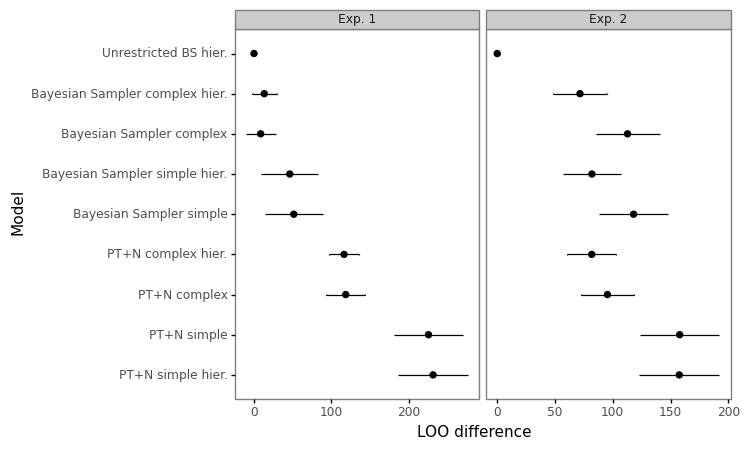
\includegraphics[width=6in]{plot_compare.png}
\caption{Model comparison results for data from Experiments 1 and 2. Error bars indicate standard errors of the estimates.}
\end{figure}

Data from Experiment 1 are only modestly informative with respect to discriminating among the models. However, data from Experiment 2 reveal a clearer winner: a hierarchical implementation of the Bayesian Sampler model that removes the restriction on \(\beta\), allowing it to range from {[}0, \(\infty\){]} (again, lower scores for \(LOO_{ic}\) are better).

Recall, this model may also be seen as a version of the PT+N theory that removes the original theory's constructive account of conditional probability judgments. Comparing predictions for conditional probability judgments from the unrestricted Bayesian Sampler model and the best-fitting PT+N model, we see that the Bayesian Sampler model better captures these judgments from Experiment 2 (trial-average-level \(R^2\) = .85 vs .73; participant-level \(R^2\) = .51 vs .45). These findings suggest that conditioning is better seen as part of the mental model than the probability judgment process.

Figure 4 shows the posterior distributions of the population-level d and d' parameters inferred from the unrestricted Bayesian Sampler model. Using data from experiment 2, population-level estimates of d and d' are greater than \(\frac{1}{3}\), outside the range implied by the assumption of ``ignorance priors'' in the Bayesian Sampler model. Parameters fit to the data from Experiment 1 are more consistent with this assumption, although a substantial proportion of individual participants' d and d' estimates also lie outside this range (13 of 59 for d, 26 of 59 for d'). The finding that there are clear differences in d and d' estimated across experiments suggest that the mental sampling processes producing estimates vary in the different conditions, either in terms of the number of samples that are drawn, the noise in reading those samples, or the form of the prior distribution assumed by participants in each context.

\begin{figure}[ht]
\centering
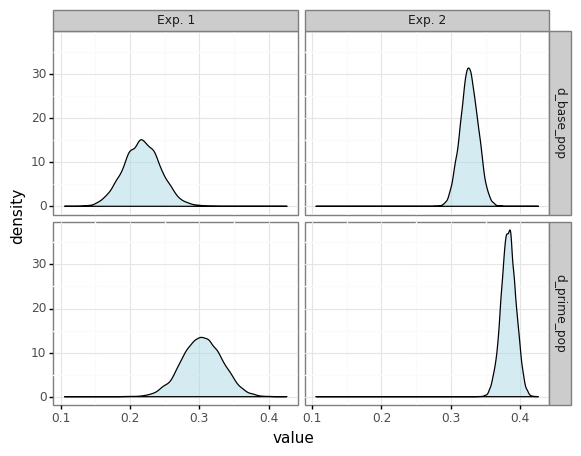
\includegraphics[width=4in]{plot_params.png}
\caption{Posterior density of population-level d and d' parameters estimated from the unrestricted hierarchical Bayesian Sampler model for data from Experiments 1 and 2.}
\end{figure}

Among the remaining models, hierarchical implementations with partial pooling outperform the unpooled corresponding models---suggesting that unpool variants of the complex models were over-penalized in the original analysis by Zhu, Sanborn, and Chater (2020). In both experiments, the simple version of the PT+N model is clearly outperformed by the other competing models. However, differences among the remaining three models are approximately within the error of the \(LOO_{ic}\) estimates. As expected, the simple variants of the models have smaller penalty terms than the complex variants.

Compared to the Bayesian Sampler model, the PT+N model with its constructive account of conditional probability judgments has a smaller penalty term despite having the same parameterization in terms of d and d'. Evidently this structural component isn't a complexifying epicycle, instead it is a prediction that constrains flexibility. However, it is one that ultimately leads to a worse-fitting model.

Perhaps surprisingly, the Bayesian Sampler with unrestricted \(\beta\) actually receives a smaller penalty term than the more restricted version of the model. This is at first unintuitive, but it illustrates how model complexity depends not only on the model and priors, but also the observed data (see Gelman, Hwang, \& Vehtari, 2014). Gelman and colleagues consider a case where a parameter is constrained to be positive and its value is estimated from data (2014). If the estimated value is some very large positive number, then the constraint won't have been very informative. But, if the estimated value is very close to zero, then the constraint that the parameter is positive will provide substantial information and the model's penalty term will therefore be smaller. Here, it seems reasonable to conjecture that because the implied d and d' estimated for this data under this model are both very near \(1/3\), the restriction results in posterior estimates of the linear parameters that are relatively far from the prior, which can result in a greater penalty.

The dependence of complexity penalties on observed data may strike some as an undesirable feature of model comparison through information criteria. Indeed, it is worth acknowledging that principled model comparison is still an area of active inquiry, with differing perspectives (e.g. Gronau \& Wagenmakers, 2019; Vehtari, Simpson, Yao, \& Gelman, 2019). Fortunately, conclusions from the comparisons here do not rest solely on differences between the models' complexity.

\begin{table}

\caption{\label{tab:table2}Bayesian model comparison results}
\centering
\resizebox{\linewidth}{!}{
\begin{tabular}[t]{lrrrrrrrr}
\toprule
\multicolumn{1}{c}{ } & \multicolumn{4}{c}{Experiment 1} & \multicolumn{4}{c}{Experiment 2} \\
\cmidrule(l{3pt}r{3pt}){2-5} \cmidrule(l{3pt}r{3pt}){6-9}
Model & $LOO_{ic}$ & Penalty & $r_{resp}$ & $r_{trial}$ & $LOO_{ic}$ & Penalty & $r_{resp}$ & $r_{trial}$\\
\midrule
\textbf{Unrestricted BS MLM} & \textbf{-1178.1} & \textbf{149.2} & \textbf{0.725} & \textbf{0.821} & \textbf{-3953.1} & \textbf{368.7} & \textbf{0.688} & \textbf{0.878}\\
Bayesian Sampler complex MLM & -1167.7 & 145.6 & 0.723 & 0.816 & -3815.4 & 399.9 & 0.675 & 0.852\\
PT+N complex & -1163.5 & 133.6 & 0.722 & 0.821 & -3768.5 & 398.2 & 0.667 & 0.840\\
Bayesian Sampler complex & -1159.5 & 149.3 & 0.723 & 0.815 & -3733.2 & 453.6 & 0.679 & 0.848\\
PT+N complex MLM & -1157.0 & 147.1 & 0.722 & 0.820 & -3796.7 & 356.1 & 0.658 & 0.835\\
\addlinespace
Bayesian Sampler simple MLM & -1149.5 & 141.0 & 0.719 & 0.810 & -3794.7 & 381.0 & 0.667 & 0.839\\
Bayesian Sampler simple & -1138.1 & 146.8 & 0.718 & 0.806 & -3722.8 & 418.9 & 0.667 & 0.831\\
PT+N simple & -1051.8 & 132.6 & 0.695 & 0.793 & -3643.0 & 319.5 & 0.619 & 0.777\\
PT+N simple MLM & -1044.7 & 137.9 & 0.695 & 0.793 & -3643.8 & 305.3 & 0.617 & 0.772\\
Relative Freq. & -746.6 & 146.8 & 0.664 & 0.737 & -1287.7 & 424.6 & 0.516 & 0.639\\
\bottomrule
\end{tabular}}
\end{table}

Finally, it is worth noting that these models provide quite strong overall fits to the data, not just for the query averages, but also for the trial averages across individual participants as seen from the correlations between predicted and observed responses in Table 2.

\hypertarget{discussion}{%
\section{Discussion}\label{discussion}}

By a fair margin, the model best accounting for the experimental data from Zhu and colleagues (2020) was a version of the Bayesian Sampler model without restriction on the range of its \(\beta\) parameters. Alternatively, this model can also be seen as a variant of the PT+N model that removes its account of conditional probability judgments. Thus, what these findings indicate most clearly is that the Bayesian Sampler theory provides a superior account of conditional probability judgments in this experimental task. In keeping with the larger theoretical framework of Bayesian cognitive science, this theory assumes that subjective probabilities underlie people's probability judgments, and that conditional probability judgments are produced by Bayesian conditioning occurring in their mental models of the events in question, rather than as arising from the probability judgment process (Chater et al., 2020; Zhu, Sanborn, \& Chater, 2020).

Findings from Zhu and colleagues' Experiment 2 do cast doubt on their proposal that the priors of the Bayesian Sampler model should reflect ``ignorance priors,'' symmetric Beta distributions with \(\beta\) \textless{} 1. As a generic prior that would be used across contexts, this class of uninformative priors has an appealing rational basis. Nevertheless, the data suggest that people may bring informative rather than ``ignorance'' priors to the probability judgment task, indicated by estimated d and d' parameters outside the {[}1, \(1/3\){]} range implied by the bridging conditions when beta is restricted \textless{} 1. One possibility is that people bring domain-specific priors to many judgment tasks, meaning that the most appropriate priors might be dictated by the context in which they make their judgments. This could potentially account for the differences in \emph{d} and \emph{d'} observed across experiments 1 and 2. In addition, these noise parameters also varied across individuals. Exploring the participant-level parameters reveals that some individuals' implied d and d' parameters were consistent with the class of ignorance priors (see supplemental materials). Further research should explore this heterogeneity within and across individuals. Unfortunately, pinning down specific components of the Bayesian Sampler model is a challenge, as the \(\beta\) and N parameters are not uniquely identifiable from judgment data of the sort examined here.

One thing this model comparison has not decided, and likely \emph{cannot} decide, is whether the distortions of probability judgments are products of mental noise or of further reasoning processes. Given their tight connections via the bridging conditions (Zhu, Sanborn, \& Chater, 2020), it may not be possible to draw decisive conclusions here. Moreover, the theories may not be in any real competition over this point: Zhu and colleagues consider that ``noise'' might give an algorithmic-level solution to the computation-level task defined by the Bayesian Sampler (2020).

Finally, some of the most interesting implications of these models go well beyond the probability judgment task itself: the models both support a probabilistic account of beliefs (Chater et al., 2020). Indeed, by representing the true subjective probabilities as a latent variable, the Bayesian modeling approach employed here allows those underlying probabilities to be inferred. Examining the model posteriors reveals these estimates often come with considerable uncertainty, but at least for some participants they can be estimated with useful levels of precision. Of course, Zhu and colleagues' (2020) experiments were never designed for this purpose. Future research could explore how these estimates might be made more reliable, and how inferences about these mental probabilities might be integrated with other Bayesian models of reasoning (e.g. Franke et al., 2016; Griffiths \& Tenenbaum, 2006; Jern, Chang, \& Kemp, 2014). One particularly promising direction could be to integrate these models with formal models of belief revision, which might then shed new light on these fundamental cognitive processes (e.g. Cook \& Lewandowsky, 2016; Jern, Chang, \& Kemp, 2014; Powell, Weisman, \& Markman, 2018).

\newpage

\hypertarget{references}{%
\section*{References}\label{references}}
\addcontentsline{toc}{section}{References}

\hypertarget{refs}{}
\begin{CSLReferences}{1}{0}
\leavevmode\hypertarget{ref-anderson1991}{}%
Anderson, J. R. (1991). The adaptive nature of human categorization. \emph{Psychological Review}, \emph{98}(3), 409--429. \url{https://doi.org/10.1037/0033-295X.98.3.409}

\leavevmode\hypertarget{ref-chater.etal2020}{}%
Chater, N., Zhu, J.-Q., Spicer, J., Sundh, J., León-Villagrá, P., \& Sanborn, A. (2020). Probabilistic {Biases Meet} the {Bayesian Brain}. \emph{Current Directions in Psychological Science}, \emph{29}(5), 506--512. \url{https://doi.org/10.1177/0963721420954801}

\leavevmode\hypertarget{ref-cook.lewandowsky2016}{}%
Cook, J., \& Lewandowsky, S. (2016). Rational {Irrationality}: {Modeling Climate Change Belief Polarization Using Bayesian Networks}. \emph{Topics in Cognitive Science}, \emph{8}(1), 160--179. \url{https://doi.org/10.1111/tops.12186}

\leavevmode\hypertarget{ref-costello.watts2014}{}%
Costello, F., \& Watts, P. (2014). Surprisingly rational: {Probability} theory plus noise explains biases in judgment. \emph{Psychological Review}, \emph{121}(3), 463--480. \url{https://doi.org/10.1037/a0037010}

\leavevmode\hypertarget{ref-costello.watts2016}{}%
Costello, F., \& Watts, P. (2016). People's conditional probability judgments follow probability theory (plus noise). \emph{Cognitive Psychology}, \emph{89}, 106--133. \url{https://doi.org/10.1016/j.cogpsych.2016.06.006}

\leavevmode\hypertarget{ref-costello.watts2017}{}%
Costello, F., \& Watts, P. (2017). Explaining {High Conjunction Fallacy Rates}: {The Probability Theory Plus Noise Account}. \emph{Journal of Behavioral Decision Making}, \emph{30}(2), 304--321. \url{https://doi.org/10.1002/bdm.1936}

\leavevmode\hypertarget{ref-costello.watts2018}{}%
Costello, F., \& Watts, P. (2018). Invariants in probabilistic reasoning. \emph{Cognitive Psychology}, \emph{100}, 1--16. \url{https://doi.org/10.1016/j.cogpsych.2017.11.003}

\leavevmode\hypertarget{ref-dasgupta.etal2017}{}%
Dasgupta, I., Schulz, E., \& Gershman, S. J. (2017). Where do hypotheses come from? \emph{Cognitive Psychology}, \emph{96}, 1--25. \url{https://doi.org/10.1016/j.cogpsych.2017.05.001}

\leavevmode\hypertarget{ref-fennell.baddeley2012}{}%
Fennell, J., \& Baddeley, R. (2012). Uncertainty plus prior equals rational bias: {An} intuitive {Bayesian} probability weighting function. \emph{Psychological Review}, \emph{119}(4), 878--887. \url{https://doi.org/10.1037/a0029346}

\leavevmode\hypertarget{ref-franke.etal2016}{}%
Franke, M., Dablander, F., Scholler, A., Bennett, E., Degen, J., Tessler, M. H., \ldots{} Goodman, N. D. (2016). What does the crowd believe? {A} hierarchical approach to estimating subjective beliefs from empirical data, 6.

\leavevmode\hypertarget{ref-gelman.etal2014a}{}%
Gelman, A., Carlin, J. B., Stern, H. S., Dunson, D. B., Vehtari, A., \& Rubin, D. B. (2014). \emph{Bayesian data analysis} (Third edition). {Boca Raton}: {CRC Press}.

\leavevmode\hypertarget{ref-gelman.etal2014}{}%
Gelman, A., Hwang, J., \& Vehtari, A. (2014). Understanding predictive information criteria for {Bayesian} models. \emph{Statistics and Computing}, \emph{24}(6), 997--1016. \url{https://doi.org/10.1007/s11222-013-9416-2}

\leavevmode\hypertarget{ref-griffiths.tenenbaum2006}{}%
Griffiths, T. L., \& Tenenbaum, J. B. (2006). Optimal {Predictions} in {Everyday Cognition}. \emph{Psychological Science}, \emph{17}(9), 767--773. \url{https://doi.org/10.1111/j.1467-9280.2006.01780.x}

\leavevmode\hypertarget{ref-gronau.wagenmakers2019}{}%
Gronau, Q. F., \& Wagenmakers, E.-J. (2019). Limitations of {Bayesian Leave}-{One}-{Out Cross}-{Validation} for {Model Selection}. \emph{Computational Brain \& Behavior}, \emph{2}(1), 1--11. \url{https://doi.org/10.1007/s42113-018-0011-7}

\leavevmode\hypertarget{ref-jaynes2003}{}%
Jaynes, E. T. (2003). \emph{Probability {Theory}: {The Logic} of {Science}}. (G. L. Bretthorst, Ed.). {Cambridge, UNITED KINGDOM}: {Cambridge University Press}.

\leavevmode\hypertarget{ref-jern.etal2014}{}%
Jern, A., Chang, K. K., \& Kemp, C. (2014). Belief polarization is not always irrational. \emph{Psychological Review}, \emph{121}(2), 206--224. \url{https://doi.org/10.1037/a0035941}

\leavevmode\hypertarget{ref-kahneman2013}{}%
Kahneman, D. (2013). \emph{Thinking, {Fast} and {Slow}} (1st edition). {New York}: {Farrar, Straus and Giroux}.

\leavevmode\hypertarget{ref-kersten.etal2004}{}%
Kersten, D., Mamassian, P., \& Yuille, A. (2004). Object {Perception} as {Bayesian Inference}. \emph{Annual Review of Psychology}, \emph{55}(1), 271--304. \url{https://doi.org/10.1146/annurev.psych.55.090902.142005}

\leavevmode\hypertarget{ref-lu.etal2012}{}%
Lu, H., Chen, D., \& Holyoak, K. J. (2012). Bayesian analogy with relational transformations. \emph{Psychological Review}, \emph{119}(3), 617--648. \url{https://doi.org/10.1037/a0028719}

\leavevmode\hypertarget{ref-mellers.etal2001}{}%
Mellers, B., Hertwig, R., \& Kahneman, D. (2001). Do {Frequency Representations Eliminate Conjunction Effects}? {An Exercise} in {Adversarial Collaboration}. \emph{Psychological Science}, \emph{12}(4), 269--275. \url{https://doi.org/10.1111/1467-9280.00350}

\leavevmode\hypertarget{ref-papaspiliopoulos.etal2007}{}%
Papaspiliopoulos, O., Roberts, G. O., \& Sköld, M. (2007). A {General Framework} for the {Parametrization} of {Hierarchical Models}. \emph{Statistical Science}, \emph{22}(1). \url{https://doi.org/10.1214/088342307000000014}

\leavevmode\hypertarget{ref-phan.etal2019}{}%
Phan, D., Pradhan, N., \& Jankowiak, M. (2019). Composable {Effects} for {Flexible} and {Accelerated Probabilistic Programming} in {NumPyro}. \emph{arXiv:1912.11554 {[}Cs, Stat{]}}. Retrieved from \url{http://arxiv.org/abs/1912.11554}

\leavevmode\hypertarget{ref-powell.etal2018}{}%
Powell, D., Weisman, K., \& Markman, E. M. (2018). Articulating lay theories through graphical models: {A} study of beliefs surrounding vaccination decisions, 6.

\leavevmode\hypertarget{ref-sides.etal2002}{}%
Sides, A., Osherson, D., Bonini, N., \& Viale, R. (2002). On the reality of the conjunction fallacy. \emph{Memory \& Cognition}, \emph{30}(2), 191--198. \url{https://doi.org/10.3758/BF03195280}

\leavevmode\hypertarget{ref-tenenbaum.etal2011}{}%
Tenenbaum, J. B., Kemp, C., Griffiths, T. L., \& Goodman, N. D. (2011). How to {Grow} a {Mind}: {Statistics}, {Structure}, and {Abstraction}. \emph{Science}, \emph{331}(6022), 1279--1285. \url{https://doi.org/10.1126/science.1192788}

\leavevmode\hypertarget{ref-tversky.kahneman1983}{}%
Tversky, A., \& Kahneman, D. (1983). Extensional {Versus Intuitive Reasoning}: {The Conjunction Fallacy} in {Probability Judgment}. \emph{Psychological Review}, \emph{90}(4), 23.

\leavevmode\hypertarget{ref-tversky.koehler1994}{}%
Tversky, A., \& Koehler, D. J. (1994). Support theory: {A} nonextensional representation of subjective probability. \emph{Psychological Review}, \emph{101}(4), 547--567. https://doi.org/\url{http://dx.doi.org.ezproxy1.lib.asu.edu/10.1037/0033-295X.101.4.547}

\leavevmode\hypertarget{ref-vehtari.etal2017}{}%
Vehtari, A., Gelman, A., \& Gabry, J. (2017). Practical {Bayesian} model evaluation using leave-one-out cross-validation and {WAIC}. \emph{Statistics and Computing}, \emph{27}(5), 1413--1432. \url{https://doi.org/10.1007/s11222-016-9696-4}

\leavevmode\hypertarget{ref-vehtari.etal2019}{}%
Vehtari, A., Simpson, D. P., Yao, Y., \& Gelman, A. (2019). Limitations of {``{Limitations} of {Bayesian Leave}-one-out {Cross}-{Validation} for {Model Selection}.''} \emph{Computational Brain \& Behavior}, \emph{2}(1), 22--27. \url{https://doi.org/10.1007/s42113-018-0020-6}

\leavevmode\hypertarget{ref-xu.tenenbaum2007}{}%
Xu, F., \& Tenenbaum, J. B. (2007). Word learning as {Bayesian} inference. \emph{Psychological Review}, \emph{114}(2), 245--272. \url{https://doi.org/10.1037/0033-295X.114.2.245}

\leavevmode\hypertarget{ref-zhu.etal2020}{}%
Zhu, J.-Q., Sanborn, A. N., \& Chater, N. (2020). The {Bayesian} sampler: {Generic Bayesian} inference causes incoherence in human probability judgments. \emph{Psychological Review}, \emph{127}(5), 719--748. \url{https://doi.org/10.1037/rev0000190}

\end{CSLReferences}


\end{document}
